% many bad boxes generated by this code
   
   \section{JOD Directory and File Layouts}\label{ss:joddirs}
   
   JOD stores J objects in binary\index{binary|see{jfiles}} \texttt{jfiles}.  
   When \hyperlink{il:newd}{newd}
    creates a dictionary it registers the location of the dictionary
    in \verb|jmaster.ijf|, see Table~\ref{tab:jmaster} on page~\pageref{tab:jmaster}, 
    and creates a set of standard directories: see 
    Figure~\ref{eps:joddirs} on page~\pageref{eps:joddirs}.
   This section describes the internal structure of JOD's binary \texttt{jfiles}.
    
  % watch the size of this graphic the placing can obscure surrounding text
  % I have previously reexported the graphic from Latexdraw to fix this
%  \begin{figure}[htbp]
%  \centering
%  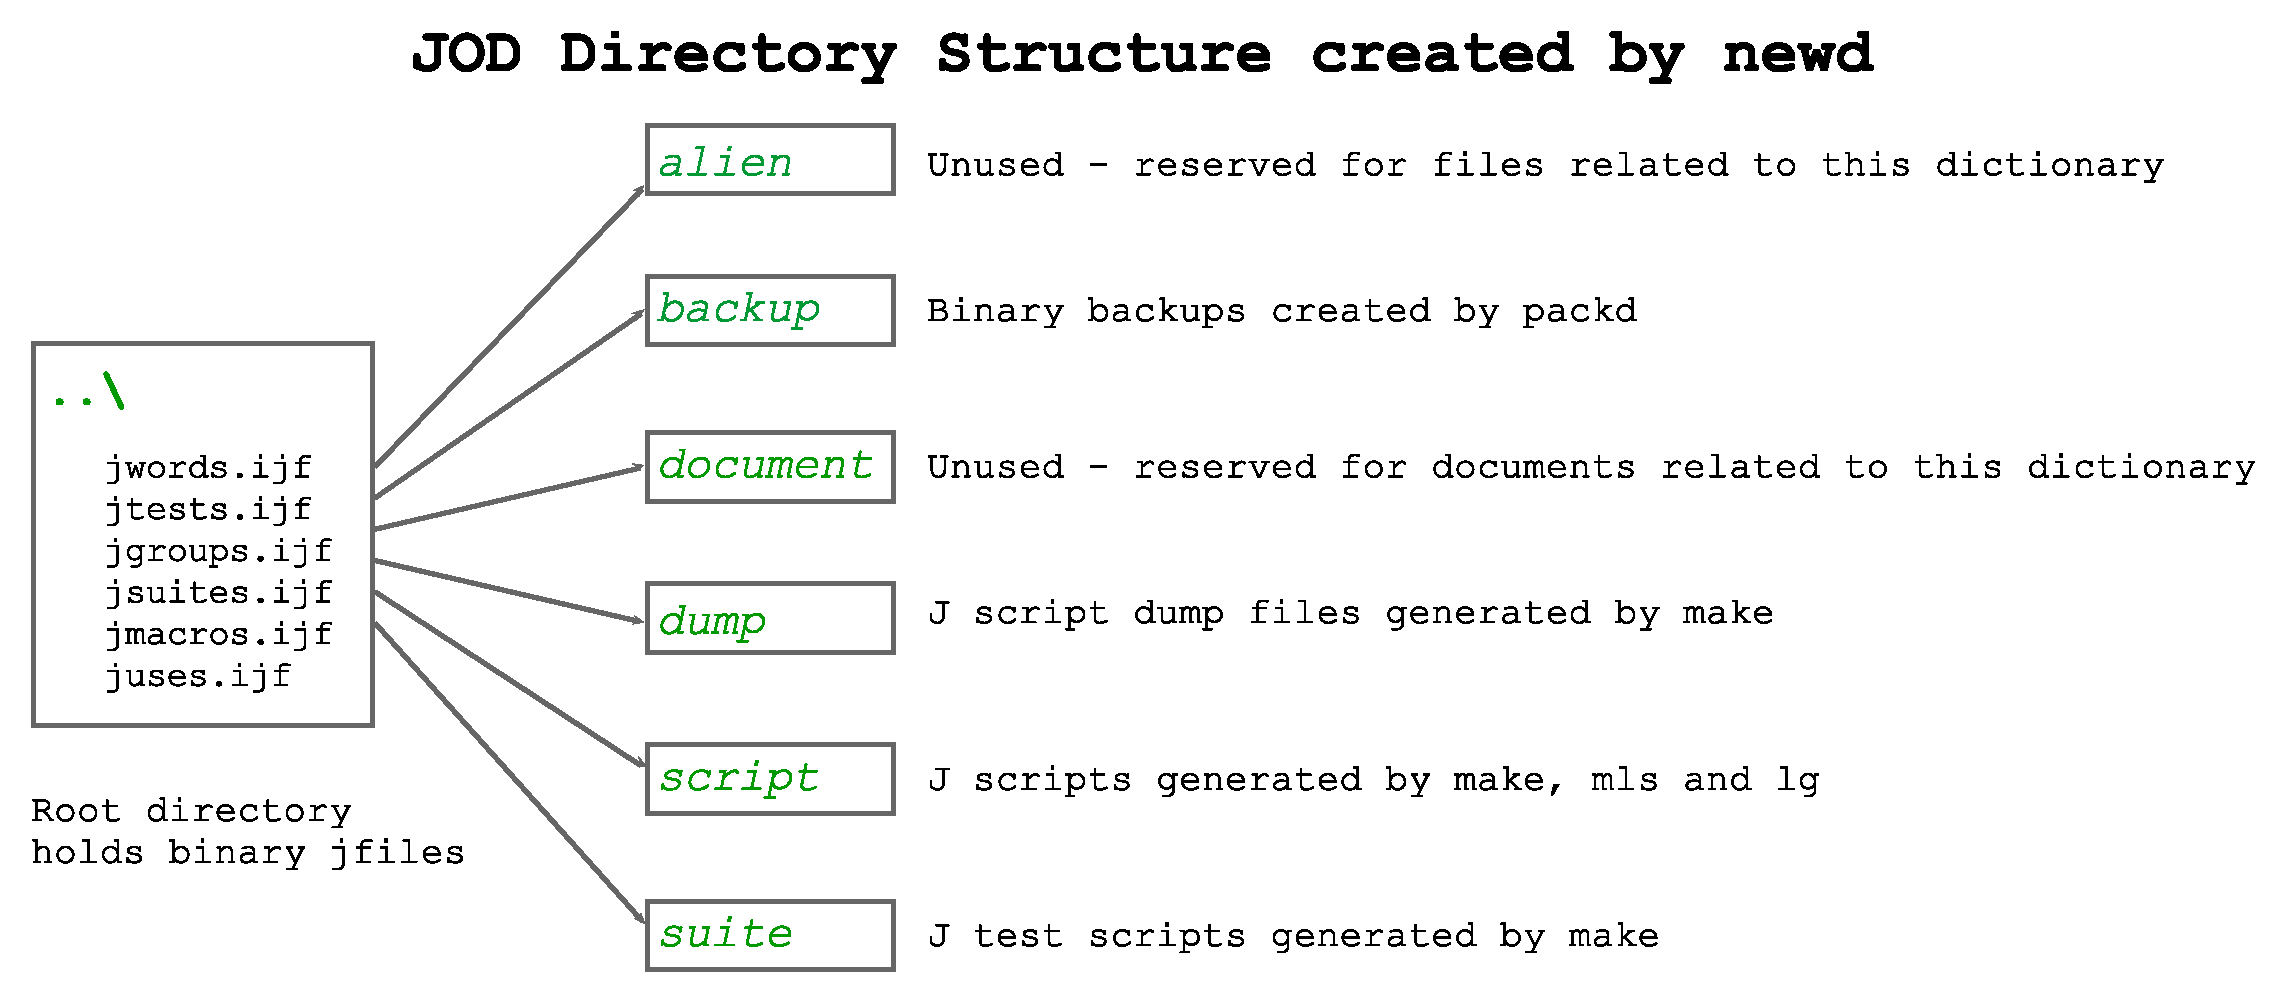
\includegraphics[width=\textwidth]{joddirectories}
%  \caption[JOD Directories]{\texttt{newd} generates this directory structure when a new JOD
%  dictionary is created. The locations of JOD directories are stored in directory objects
%  when dictionaries are opened.}
%   \label{eps:joddirs}
%   \end{figure}

% similar graphic generated with the dirtree package - allows
% cross references to other parts of the document

\begin{figure}[htbp]\index{directories!JOD Directory Structure}
\begin{center} \large
JOD Directory Structure created by \hyperlink{il:newd}{\texttt{newd}} \textbf{\textcolor{CodeComment}{\texttt{'name';'\ldots{}/'}}} \\
\end{center} \normalsize
\dirtree{%
.1 \textbf{\textcolor{CodeComment}{\ldots{}/name}} 
\begin{minipage}[t]{0.8\textwidth}
\textrm{The dictionary root directory holds binary \texttt{jfiles}, see section~\ref{ss:joddirs}
on page~\pageref{ss:joddirs}{.}}\\
jwords{.}ijf, jtests{.}ijf \\
jgroups{.}ijf, jsuites{.}ijf \\
jmacros{.}ijf \\
juses{.}ijf \\
\end{minipage}.
.3 \textbf{\textcolor{CodeComment}{name/alien}} \begin{minipage}[t]{0.8\textwidth}
\textrm{Unused --- reserved for files related to this dictionary{.}}
\end{minipage}.
.3 \textbf{\textcolor{CodeComment}{name/backup}} \begin{minipage}[t]{0.8\textwidth}
\textrm{Binary backups created by \hyperlink{il:packd}{\texttt{packd}} (\pageref{ss:packd}){.}}
\end{minipage}.
.3 \textbf{\textcolor{CodeComment}{name/document}} \begin{minipage}[t]{0.8\textwidth}
\textrm{Unused --- reserved for documents related to this dictionary{.}}
\end{minipage}.
.3 \textbf{\textcolor{CodeComment}{name/dump}} \begin{minipage}[t]{0.8\textwidth}
\textrm{J dump script files generated by \hyperlink{il:make}{\texttt{make}} (\pageref{ss:make}){.}}
\end{minipage}.
.3 \textbf{\textcolor{CodeComment}{name/script}} \begin{minipage}[t]{0.8\textwidth}
\textrm{J script files generated by \hyperlink{il:make}{\texttt{make}}, \hyperlink{il:mls}{\texttt{mls}} and \hyperlink{il:lg}{\texttt{lg}} (\pageref{ss:make},~\pageref{ss:mls},~\pageref{ss:lg}){.}}
\end{minipage}.
.3 \textbf{\textcolor{CodeComment}{name/suite}} \begin{minipage}[t]{0.8\textwidth}
\textrm{J test scripts generated by \hyperlink{il:make}{\texttt{make}} (\pageref{ss:make}){.}}
\end{minipage}.
}
\caption[JOD Directories]{\texttt{newd} generates this directory structure when a new JOD
  dictionary is created. The locations of JOD directories are stored in directory objects
  when dictionaries are opened.}
\label{eps:joddirs}
\end{figure}
   
   \subsection{Master File --- \texttt{jmaster.ijf}}\index{master file}
   
   \texttt{jmaster.ijf} is a binary component \texttt{jfile}.  To use
   \texttt{jfiles} you load or require the standard \texttt{jfiles} script.
    
   \texttt{jmaster.ijf} is an index of currently registered dictionaries and standard dictionary metadata. 
   The component layout  of \texttt{jmaster.ijf} is given in Table~\ref{tab:jmaster} on page~\pageref{tab:jmaster}.
   
\begin{table}[htbp]
  \centering
   \scriptsize
 { \renewcommand{\arraystretch}{\JFILESARP}
\begin{tabular}{|l|l|p{\JFILESTPW\textwidth}|} \hline
      \multicolumn{3}{|c|}{\large\textbf{\texttt{jmaster.ijf}}\T\B}\\ \hline
      \multicolumn{1}{|c|}{\textbf{Component}\T} &
      \multicolumn{1}{|c|}{\textbf{Hungarian}}  &
      \multicolumn{1}{|c|}{\textbf{Description}\B} \\ \hline
$c_{0}$ &  \texttt{(pa;il)}  & 
  \begin{tabular}{p{\JFILESTPS\textwidth}}
	Use bit and last master change. \\
	\\
	The use bit is set by all processes that update this
  file - while set the use bit blocks other dictionary tasks
  from updating this file. \\
  \end{tabular} \\ \hline
$c_{1}$  & \texttt{(cl;i,X)} & 
  \begin{tabular}{p{\JFILESTPS\textwidth}}
  Version \texttt{m.m.p} character, build count and unique master file id. \\
  \end{tabular} \\ \hline 
$c_{2}$  &  \texttt{bt}   &  
   \begin{tabular}{p{\JFILESTPS\textwidth}}
   Dictionary names, numbers, directories and read-write status. \\
   \\
When a dictionary is opened for update (\texttt{READWRITE} default) 
by \hyperlink{il:od}{\texttt{od}} (pp.~\pageref{ss:od}) the status is set and stays on
until closed by \texttt{od}. This blocks all other dictionary tasks from updating the dictionary. This
harsh treatment prevents garbled files. Dictionaries can also be opened read only. This allows
multiple readers but no writers. \\
   \end{tabular} \\ \hline 
$c_{3}$  &  \texttt{bt}   &  
   \begin{tabular}{p{\JFILESTPS\textwidth}}
   Previous master directory. \\
   \\
   Essentially a copy of component two less at most one deleted or new dictionary. \\
   \end{tabular} \\ \hline 
$c_{4}\rightarrow c_{6}$ &  &     
   \begin{tabular}{p{\JFILESTPS\textwidth}}
   \emph{Reserved.} \\
   \end{tabular} \\ \hline 
$c_{7}$  &  \texttt{bt}   &   
   \begin{tabular}{p{\JFILESTPS\textwidth}}
   Active dictionary parameters. \\
   \\
   \verb|0 { - blcl| ; parameter names \\
   \verb|1 { - blcl| ; short parameter explanation \\
   \verb|2 { - bluu| ; default values \\
   \end{tabular} \\ \hline 
$c_{8}$  &  \texttt{bt}   & 
    \begin{tabular}{p{\JFILESTPS\textwidth}}
    Copy of active dictionary parameters. \\
    \end{tabular} \\ \hline 
$c_{9}$  &  \texttt{bt}   & 
    \begin{tabular}{p{\JFILESTPS\textwidth}}
    Default dictionary parameters. \\
    \end{tabular} \\ \hline 
$c_{10}$  &  \texttt{Xl}   & 
    \begin{tabular}{p{\JFILESTPS\textwidth}}
     Dictionary log. \\
     \\
The dictionary log is a simple, (append only), list of all the extended dictionary
numbers (\texttt{DIDNUM}s) that\index{DIDNUM} have ever been registered. When a dictionary is registered it is appended to this list.
If it is unregistered and then re-registered the same dictionary number will appear more than once.
I don't expect  this list to be very large. Hundreds, maybe thousands, over the lifetime of the master file. \\
    \end{tabular} \\ \hline 
\end{tabular}
}
\caption{\texttt{jmaster.ijf} file\index{jfiles!\texttt{jmaster.ijf}} component layout}
\label{tab:jmaster}
\end{table}
      
   \subsection{Words File --- \texttt{jwords.ijf}}

 \texttt{jwords.ijf} is a binary component \texttt{jfile}. 
 \texttt{jwords.ijf} contains word definitions and metadata. The component layout 
 of \texttt{jwords.ijf} is given in Table~\ref{tab:jwords} on page~\pageref{tab:jwords}.
   
\begin{table}[htbp]
  \centering
   \scriptsize
   { \renewcommand{\arraystretch}{\JFILESARP}
   \begin{tabular}{|l|l|p{\JFILESTPW\textwidth}|} \hline
       \multicolumn{3}{|c|}{\large\textbf{\texttt{jwords.ijf}}\T\B}\\ \hline
      \multicolumn{1}{|c|}{\textbf{Component}\T} &
      \multicolumn{1}{|c|}{\textbf{Hungarian}}  &
      \multicolumn{1}{|c|}{\textbf{Description}\B} \\ \hline
 $c_{0}$ &  \texttt{blnl}  & 
  \begin{tabular}{p{\JFILESTPS\textwidth}}
	Length and last directory change. \\
  \end{tabular} \\ \hline
$c_{1}$  & \texttt{fl} & 
  \begin{tabular}{p{\JFILESTPS\textwidth}}
   Pack count and last backup or restore timestamp.
   Pack count prefixes backup and dump files. \\
  \end{tabular} \\ \hline 
$c_{2}$  &  \texttt{cl}   &  
   \begin{tabular}{p{\JFILESTPS\textwidth}}
    Dictionary documentation \hyperlink{il:newd}{\texttt{newd}}, \hyperlink{il:regd}{\texttt{regd}}. (pp.~\pageref{ss:newd},\pageref{ss:regd})\\ 
   \end{tabular} \\ \hline 
$c_{3}$  &  \texttt{bluu}   &  
   \begin{tabular}{p{\JFILESTPS\textwidth}}
   Dictionary parameters. \\
\verb|0  { - cl| ; dictionary name \\
\verb|1  { - Xa| ; dictionary number \texttt{DIDNUM} (\emph{extended precision}) \\
\verb|2  { - il| ; dictionary creation date \\
\verb|3  { - il| ; last dump date \textit{(not updated)} \\
\verb|4  { - cl| ; script directory \\
\verb|5  { - cl| ; suite directory \\
\verb|6  { - cl| ; macro directory \\
\verb|7  { - cl| ; document directory \\
\verb|8  { - cl| ; dump directory \\
\verb|9  { - cl| ; alien directory \\
\verb|10 { - cl| ; J version that created dictionary \\
\verb|11 { - ia| ; J system code that created dictionary \\
\verb|12 { - uu| ; unused - \textit{reserved} \\
\verb|13 { - bt| ; user dictionary parameters see: \hyperlink{il:jmaster}{\texttt{jmaster.ijf}} (pp.~\pageref{tab:jmaster}). \\
\hspace{\JFILESHSP}  \verb|0 { cl| ; parameter \\
\hspace{\JFILESHSP}  \verb|1 { uu| ; value \\
   \end{tabular} \\ \hline 
      & &
   \begin{tabular}{p{\JFILESTPS\textwidth}}
   Main inverted items, $c_{4}\rightarrow c_{11}$ have the same length. \\
   \end{tabular} \\ \hline
$c_{4}$ & \texttt{blcl} &     
   \begin{tabular}{p{\JFILESTPS\textwidth}}
   Word list (main index 1).\\
   \end{tabular} \\ \hline 
$c_{5}$  &  \texttt{il}   &   
   \begin{tabular}{p{\JFILESTPS\textwidth}}
   Word components (main index 2).\\
   \end{tabular} \\ \hline 
$c_{6}$  &  \texttt{il}   & 
    \begin{tabular}{p{\JFILESTPS\textwidth}}
    Name class list.\\
    \end{tabular} \\ \hline 
$c_{7}$  &  \texttt{fl}   & 
    \begin{tabular}{p{\JFILESTPS\textwidth}}
    Last put date list \texttt{yyyymmdd.fd} (fractional day). \\
    \end{tabular} \\ \hline 
$c_{8}$  &  \texttt{fl}   & 
    \begin{tabular}{p{\JFILESTPS\textwidth}}
    Creation put list \texttt{yyyymmdd.fd} (fractional day).\\
    \end{tabular} \\ \hline 
$c_{9}$  &  \texttt{il}   & 
    \begin{tabular}{p{\JFILESTPS\textwidth}}
    Word size in bytes.\\
    \end{tabular} \\ \hline 
$c_{10}$  &     & 
    \begin{tabular}{p{\JFILESTPS\textwidth}}
    \textit{Reserved.}\\
    \end{tabular} \\ \hline 
$c_{11}$  &  \texttt{blcl}   & 
    \begin{tabular}{p{\JFILESTPS\textwidth}}
    Short word explanations.\\
    \end{tabular} \\ \hline 
$c_{12}$ &  \texttt{cl} &     
   \begin{tabular}{p{\JFILESTPS\textwidth}}
   J version string \verb|9!:14 ''| or empty.\\
   \end{tabular} \\ \hline 
$c_{13}\rightarrow c_{38}$    & &
   \begin{tabular}{p{\JFILESTPS\textwidth}}
    \textit{Reserved.} The remaining component pairs contain word data.
    The word names match the entries in the word index list.\\
   \end{tabular} \\ \hline
$c_{39}$  &  \texttt{bluu}   & 
    \begin{tabular}{p{\JFILESTPS\textwidth}}
    Word definition.\\
    \verb|0 { - cl| ; word name \\
    \verb|1 { - ia| ; name class \\
    \verb|2 { - cl| \argsep \texttt{uu} ; word value: nouns binary, 
    all others character lists \\
    \end{tabular} \\ \hline 
$c_{40}$  &  \texttt{bluu}   & 
    \begin{tabular}{p{\JFILESTPS\textwidth}}
    Word documentation and other.\\
    \verb|0 { - cl| ; word name \\
    \verb|1 { - uu| ; unused - \emph{reserved} \\
    \verb|2 { - uu| ; unused - \emph{reserved} \\
    \verb|3 { - cl| ; text documentation \\
    \end{tabular} \\ \hline 
$c_{41}$  &  \texttt{bluu}   & 
    \begin{tabular}{p{\JFILESTPS\textwidth}}
    Like $c_{39}$ \\
    \end{tabular} \\ \hline 
$c_{42}$  &  \texttt{bluu}   & 
    \begin{tabular}{p{\JFILESTPS\textwidth}}
    Like $c_{40}$ \\
    \end{tabular} \\ \hline   
  \ldots & \ldots & \ldots \\ \hline
$c_{n}$  &  \ldots   & 
    \begin{tabular}{p{\JFILESTPS\textwidth}}
    Like $c_{n-2}$ \\
    \end{tabular} \\ \hline   
\end{tabular}
}
\caption{\texttt{jwords.ijf} file\index{jfiles!\texttt{jwords.ijf}} component layout}
\label{tab:jwords}
\end{table}
   
   \subsection{Tests File --- \texttt{jtests.ijf}}

\texttt{jtests.ijf} is a binary component \texttt{jfile}.  
\texttt{jtests.ijf} contains test definitions and metadata. The component layout 
of \texttt{jtests.ijf} is given in Table~\ref{tab:jtests} on page~\pageref{tab:jtests}.
   
\begin{table}[htbp]
  \centering
   \scriptsize
   { \renewcommand{\arraystretch}{\JFILESARP}
   \begin{tabular}{|l|l|p{\JFILESTPW\textwidth}|} \hline
      \multicolumn{3}{|c|}{\large\textbf{\texttt{jtests.ijf}}\T\B}\\ \hline
      \multicolumn{1}{|c|}{\textbf{Component}\T} &
      \multicolumn{1}{|c|}{\textbf{Hungarian}}  &
      \multicolumn{1}{|c|}{\textbf{Description}\B} \\ \hline
  $c_{0}$ &  \texttt{blnl}  & 
  \begin{tabular}{p{\JFILESTPS\textwidth}}
	Length and last directory change. \\
  \end{tabular} \\ \hline
$c_{1}\rightarrow c_{3}$ &  & 
  \begin{tabular}{p{\JFILESTPS\textwidth}}
  \emph{Reserved.} \\
  \end{tabular} \\ \hline 
  & & \\ \hline
  & &
   \begin{tabular}{p{\JFILESTPS\textwidth}}
   Main inverted items, $c_{4}\rightarrow c_{11}$ have the same length. \\
   \end{tabular} \\ \hline
$c_{4}$ & \texttt{blcl} &     
   \begin{tabular}{p{\JFILESTPS\textwidth}}
   Test list (main index 1).\\
   \end{tabular} \\ \hline 
$c_{5}$  &  \texttt{il}   &   
   \begin{tabular}{p{\JFILESTPS\textwidth}}
   Test components (main index 2).\\
   \end{tabular} \\ \hline 
$c_{6}$  &    & 
    \begin{tabular}{p{\JFILESTPS\textwidth}}
    Reserved to match \texttt{jwords.ijf}.\\
    \end{tabular} \\ \hline 
$c_{7}$  &  \texttt{fl}   & 
    \begin{tabular}{p{\JFILESTPS\textwidth}}
    Last put date list \texttt{yyyymmdd.fd} (fractional day). \\
    \end{tabular} \\ \hline 
$c_{8}$  &  \texttt{fl}   & 
    \begin{tabular}{p{\JFILESTPS\textwidth}}
    Creation put list \texttt{yyyymmdd.fd} (fractional day).\\
    \end{tabular} \\ \hline 
$c_{9}$  &  \texttt{il}   & 
    \begin{tabular}{p{\JFILESTPS\textwidth}}
    Test size in bytes.\\
    \end{tabular} \\ \hline 
$c_{10}$  &     & 
    \begin{tabular}{p{\JFILESTPS\textwidth}}
    \emph{Reserved.}\\
    \end{tabular} \\ \hline 
$c_{11}$  &  \texttt{blcl}   & 
    \begin{tabular}{p{\JFILESTPS\textwidth}}
    Short test explanations.\\
    \end{tabular} \\ \hline 
$c_{12}\rightarrow c_{38}$ &  &     
   \begin{tabular}{p{\JFILESTPS\textwidth}}
   \emph{Reserved.} \\
   \end{tabular} \\ \hline 
    & & \\ \hline
    & &
   \begin{tabular}{p{\JFILESTPS\textwidth}}
    The remaining component pairs contain test data.
    The test names match the entries in the test index $c_{4}$ list.\\
   \end{tabular} \\ \hline
$c_{39}$  &  \texttt{blcl}   & 
    \begin{tabular}{p{\JFILESTPS\textwidth}}
    Test definition.\\
    \\
    \verb|0 { - cl| ; test name \\
    \verb|1 { - cl| ; test value \\
    \end{tabular} \\ \hline 
$c_{40}$  &  \texttt{bluu}   & 
    \begin{tabular}{p{\JFILESTPS\textwidth}}
    Test documentation and other.\\
    \\
    \verb|0 { - cl| ; test name \\
    \verb|1 { - uu| ; unused - \emph{reserved} \\
    \verb|2 { - uu| ; unused - \emph{reserved} \\
    \verb|3 { - cl| ; text documentation \\
    \end{tabular} \\ \hline 
$c_{41}$  &  \texttt{blcl}   & 
    \begin{tabular}{p{\JFILESTPS\textwidth}}
    Like $c_{39}$ \\
    \end{tabular} \\ \hline 
$c_{42}$  &  \texttt{bluu}   & 
    \begin{tabular}{p{\JFILESTPS\textwidth}}
    Like $c_{40}$ \\
    \end{tabular} \\ \hline   
  \ldots & \ldots & \ldots \\ \hline
$c_{n}$  &  \ldots   & 
    \begin{tabular}{p{\JFILESTPS\textwidth}}
    Like $c_{n-2}$ \\
    \end{tabular} \\ \hline  
\end{tabular}
}
\caption{\texttt{jtests.ijf} file\index{jfiles!\texttt{jtests.ijf}} component layout}
\label{tab:jtests}
\end{table}
 
   \subsection{Groups File --- \texttt{jgroups.ijf}}
   
\texttt{jgroups.ijf} is a binary component \texttt{jfile}.  
\texttt{jgroups.ijf} contains group definitions and group metadata. The component layout 
of \texttt{jgroups.ijf} is given in Table~\ref{tab:jgroups} on page~\pageref{tab:jgroups}.

\begin{table}[htbp]
  \centering
   \scriptsize
   { \renewcommand{\arraystretch}{\JFILESARP}
   \begin{tabular}{|l|l|p{\JFILESTPW\textwidth}|} \hline
       \multicolumn{3}{|c|}{\large\textbf{\texttt{jgroups.ijf}}\T\B}\\ \hline
      \multicolumn{1}{|c|}{\textbf{Component}\T} &
      \multicolumn{1}{|c|}{\textbf{Hungarian}}  &
      \multicolumn{1}{|c|}{\textbf{Description}\B} \\ \hline
    $c_{0}$ &  \texttt{blnl}  & 
  \begin{tabular}{p{\JFILESTPS\textwidth}}
	Group count and last directory change. \\
  \end{tabular} \\ \hline
$c_{1}\rightarrow c_{3}$ &  & 
  \begin{tabular}{p{\JFILESTPS\textwidth}}
  \emph{Reserved.} \\
  \end{tabular} \\ \hline 
  & & \\ \hline
  & &
   \begin{tabular}{p{\JFILESTPS\textwidth}}
   Main inverted items, $c_{4}\rightarrow c_{11}$ have the same length. \\
   \end{tabular} \\ \hline
$c_{4}$ & \texttt{blcl} &     
   \begin{tabular}{p{\JFILESTPS\textwidth}}
   Group list (main index 1).\\
   \end{tabular} \\ \hline 
$c_{5}$  &  \texttt{il}   &   
   \begin{tabular}{p{\JFILESTPS\textwidth}}
   Group components (main index 2).\\
   \end{tabular} \\ \hline 
$c_{6}$  &    & 
    \begin{tabular}{p{\JFILESTPS\textwidth}}
    Reserved to match \texttt{jwords.ijf}.\\
    \end{tabular} \\ \hline 
$c_{7}$  &  \texttt{fl}   & 
    \begin{tabular}{p{\JFILESTPS\textwidth}}
    Last put date list \texttt{yyyymmdd.fd} (fractional day). \\
    \end{tabular} \\ \hline 
$c_{8}$  &  \texttt{fl}   & 
    \begin{tabular}{p{\JFILESTPS\textwidth}}
    Creation put list \texttt{yyyymmdd.fd} (fractional day).\\
    \end{tabular} \\ \hline 
$c_{9}\rightarrow c_{10}$ &    & 
    \begin{tabular}{p{\JFILESTPS\textwidth}}
    \emph{Reserved.}\\
    \end{tabular} \\ \hline 
$c_{11}$  &  \texttt{blcl}   & 
    \begin{tabular}{p{\JFILESTPS\textwidth}}
    Short group explanations.\\
    \end{tabular} \\ \hline 
$c_{12}\rightarrow c_{38}$ &  &     
   \begin{tabular}{p{\JFILESTPS\textwidth}}
   \emph{Reserved.} \\
   \end{tabular} \\ \hline 
    & & \\ \hline
    & &
   \begin{tabular}{p{\JFILESTPS\textwidth}}
    The remaining component pairs contain group data.
    The group names match the entries in the group index $c_{4}$ list.\\
   \end{tabular} \\ \hline
$c_{39}$  &  \texttt{bluu}   & 
    \begin{tabular}{p{\JFILESTPS\textwidth}}
    Group definition.\\
    \\
    \verb|0 { - cl| ; group name \\
    \verb|1 { - cl| ; group prefix script \\
    \verb|2 { - blcl| ; group content list \\
    \end{tabular} \\ \hline 
$c_{40}$  &  \texttt{bluu}   & 
    \begin{tabular}{p{\JFILESTPS\textwidth}}
    Group documentation and other.\\
    \\
    \verb|0 { - cl| ; group name \\
    \verb|1 { - uu| ; unused - \emph{reserved} \\
    \verb|2 { - uu| ; unused - \emph{reserved} \\
    \verb|3 { - cl| ; text documentation \\
    \end{tabular} \\ \hline 
$c_{41}$  &  \texttt{bluu}   & 
    \begin{tabular}{p{\JFILESTPS\textwidth}}
    Like $c_{39}$ \\
    \end{tabular} \\ \hline 
$c_{42}$  &  \texttt{bluu}   & 
    \begin{tabular}{p{\JFILESTPS\textwidth}}
    Like $c_{40}$ \\
    \end{tabular} \\ \hline   
  \ldots & \ldots & \ldots \\ \hline
$c_{n}$  &  \ldots   & 
    \begin{tabular}{p{\JFILESTPS\textwidth}}
    Like $c_{n-2}$ \\
    \end{tabular} \\ \hline      
\end{tabular}	
}
\caption{\texttt{jgroups.ijf} file\index{jfiles!\texttt{jgroups.ijf}} component layout}
\label{tab:jgroups}
\end{table}
   
   \subsection{Suites File --- \texttt{jsuites.ijf}}
   
\texttt{jsuites.ijf} is a binary component \texttt{jfile}.  
\texttt{jsuites.ijf} contains test suite definitions and test suite metadata. 
The component layout of \texttt{jsuites.ijf} is given in Table~\ref{tab:jsuites} on page~\pageref{tab:jsuites}.

\begin{table}[htbp]
  \centering
   \scriptsize
 { \renewcommand{\arraystretch}{\JFILESARP}
   \begin{tabular}{|l|l|p{\JFILESTPW\textwidth}|} \hline
       \multicolumn{3}{|c|}{\large\textbf{\texttt{jsuites.ijf}}\T\B}\\ \hline
      \multicolumn{1}{|c|}{\textbf{Component}\T} &
      \multicolumn{1}{|c|}{\textbf{Hungarian}}  &
      \multicolumn{1}{|c|}{\textbf{Description}\B} \\ \hline
      $c_{0}$ &  \texttt{blnl}  & 
  \begin{tabular}{p{\JFILESTPS\textwidth}}
	Suite count and last directory change. \\
  \end{tabular} \\ \hline
$c_{1}\rightarrow c_{3}$ &  & 
  \begin{tabular}{p{\JFILESTPS\textwidth}}
  \emph{Reserved.} \\
  \end{tabular} \\ \hline 
  & & \\ \hline
  & &
   \begin{tabular}{p{\JFILESTPS\textwidth}}
   Main inverted items, $c_{4}\rightarrow c_{11}$ have the same length. \\
   \end{tabular} \\ \hline
$c_{4}$ & \texttt{blcl} &     
   \begin{tabular}{p{\JFILESTPS\textwidth}}
   Suite list (main index 1).\\
   \end{tabular} \\ \hline 
$c_{5}$  &  \texttt{il}   &   
   \begin{tabular}{p{\JFILESTPS\textwidth}}
   Suite components (main index 2).\\
   \end{tabular} \\ \hline 
$c_{6}$  &    & 
    \begin{tabular}{p{\JFILESTPS\textwidth}}
    Reserved to match \texttt{jwords.ijf}.\\
    \end{tabular} \\ \hline 
$c_{7}$  &  \texttt{fl}   & 
    \begin{tabular}{p{\JFILESTPS\textwidth}}
    Last put date list \texttt{yyyymmdd.fd} (fractional day). \\
    \end{tabular} \\ \hline 
$c_{8}$  &  \texttt{fl}   & 
    \begin{tabular}{p{\JFILESTPS\textwidth}}
    Creation put list \texttt{yyyymmdd.fd} (fractional day).\\
    \end{tabular} \\ \hline 
$c_{9}\rightarrow c_{10}$ &    & 
    \begin{tabular}{p{\JFILESTPS\textwidth}}
    \emph{Reserved.}\\
    \end{tabular} \\ \hline 
$c_{11}$  &  \texttt{blcl}   & 
    \begin{tabular}{p{\JFILESTPS\textwidth}}
    Short suite explanations.\\
    \end{tabular} \\ \hline 
$c_{12}\rightarrow c_{38}$ &  &     
   \begin{tabular}{p{\JFILESTPS\textwidth}}
   \emph{Reserved.} \\
   \end{tabular} \\ \hline 
    & & \\ \hline
    & &
   \begin{tabular}{p{\JFILESTPS\textwidth}}
    The remaining component pairs contain suite data.
    The suite names match the entries in the suite index $c_{4}$ list.\\
   \end{tabular} \\ \hline
$c_{39}$  &  \texttt{bluu}   & 
    \begin{tabular}{p{\JFILESTPS\textwidth}}
    Suite definition.\\
    \\
    \verb|0 { - cl| ; suite name \\
    \verb|1 { - cl| ; suite prefix script \\
    \verb|2 { - blcl| ; suite content list \\
    \end{tabular} \\ \hline 
$c_{40}$  &  \texttt{bluu}   & 
    \begin{tabular}{p{\JFILESTPS\textwidth}}
    Suite documentation and other.\\
    \\
    \verb|0 { - cl| ; suite name \\
    \verb|1 { - uu| ; unused - \emph{reserved} \\
    \verb|2 { - uu| ; unused - \emph{reserved} \\
    \verb|3 { - cl| ; text documentation \\
    \end{tabular} \\ \hline 
$c_{41}$  &  \texttt{bluu}   & 
    \begin{tabular}{p{\JFILESTPS\textwidth}}
    Like $c_{39}$ \\
    \end{tabular} \\ \hline 
$c_{42}$  &  \texttt{bluu}   & 
    \begin{tabular}{p{\JFILESTPS\textwidth}}
    Like $c_{40}$ \\
    \end{tabular} \\ \hline   
  \ldots & \ldots & \ldots \\ \hline
$c_{n}$  &  \ldots   & 
    \begin{tabular}{p{\JFILESTPS\textwidth}}
    Like $c_{n-2}$ \\
    \end{tabular} \\ \hline         
\end{tabular}
}
\caption{\texttt{jsuites.ijf} file\index{jfiles!\texttt{jsuites.ijf}} component layout}
\label{tab:jsuites}
\end{table}
   
   \subsection{Macros File --- \texttt{jmacros.ijf}}
   
\texttt{jmacros.ijf} is a binary component \texttt{jfile}.  
\texttt{jmacros.ijf} contains macro script definitions and macro script metadata. 
The component layout of \texttt{jmacros.ijf} is given in Table~\ref{tab:jmacros} on page~\pageref{tab:jmacros}.

\begin{table}[htbp]
  \centering
   \scriptsize
 { \renewcommand{\arraystretch}{\JFILESARP}
   \begin{tabular}{|l|l|p{\JFILESTPW\textwidth}|} \hline
        \multicolumn{3}{|c|}{\large\textbf{\texttt{jmacros.ijf}}\T\B}\\ \hline
      \multicolumn{1}{|c|}{\textbf{Component}\T} &
      \multicolumn{1}{|c|}{\textbf{Hungarian}}  &
      \multicolumn{1}{|c|}{\textbf{Description}\B} \\ \hline
$c_{0}$ &  \texttt{blnl}  & 
  \begin{tabular}{p{\JFILESTPS\textwidth}}
	Macro count and last directory change. \\
  \end{tabular} \\ \hline
$c_{1}\rightarrow c_{3}$ &  & 
  \begin{tabular}{p{\JFILESTPS\textwidth}}
  \emph{Reserved.} \\
  \end{tabular} \\ \hline 
  & & \\ \hline
  & &
   \begin{tabular}{p{\JFILESTPS\textwidth}}
   Main inverted items, $c_{4}\rightarrow c_{11}$ have the same length. \\
   \end{tabular} \\ \hline
$c_{4}$ & \texttt{blcl} &     
   \begin{tabular}{p{\JFILESTPS\textwidth}}
   Macro list (main index 1).\\
   \end{tabular} \\ \hline 
$c_{5}$  &  \texttt{il}   &   
   \begin{tabular}{p{\JFILESTPS\textwidth}}
   Macro components (main index 2).\\
   \end{tabular} \\ \hline 
$c_{6}$  &    & 
    \begin{tabular}{p{\JFILESTPS\textwidth}}
    Reserved to match \texttt{jwords.ijf}.\\
    \end{tabular} \\ \hline 
$c_{7}$  &  \texttt{fl}   & 
    \begin{tabular}{p{\JFILESTPS\textwidth}}
    Last put date list \texttt{yyyymmdd.fd} (fractional day). \\
    \end{tabular} \\ \hline 
$c_{8}$  &  \texttt{fl}   & 
    \begin{tabular}{p{\JFILESTPS\textwidth}}
    Creation put list \texttt{yyyymmdd.fd} (fractional day).\\
    \end{tabular} \\ \hline 
$c_{9}$ &  \texttt{fl}  & 
    \begin{tabular}{p{\JFILESTPS\textwidth}}
    Macro size in bytes.\\
    \end{tabular} \\ \hline
$c_{10}$ &  &     
   \begin{tabular}{p{\JFILESTPS\textwidth}}
   \emph{Reserved.} \\
   \end{tabular} \\ \hline  
$c_{11}$  &  \texttt{blcl}   & 
    \begin{tabular}{p{\JFILESTPS\textwidth}}
    Short macro explanations.\\
    \end{tabular} \\ \hline 
$c_{12}\rightarrow c_{38}$ &  &     
   \begin{tabular}{p{\JFILESTPS\textwidth}}
   \emph{Reserved.} \\
   \end{tabular} \\ \hline 
    & & \\ \hline
    & &
   \begin{tabular}{p{\JFILESTPS\textwidth}}
    The remaining component pairs contain macro data.
    The macro names match the entries in the macro index $c_{4}$ list.\\
   \end{tabular} \\ \hline
$c_{39}$  &  \texttt{blcl}   & 
    \begin{tabular}{p{\JFILESTPS\textwidth}}
    Macro definition.\\
    \\
    \verb|0 { - cl| ; macro name \\
    \verb|1 { - cl| ; macro script \\
    \end{tabular} \\ \hline 
$c_{40}$  &  \texttt{bluu}   & 
    \begin{tabular}{p{\JFILESTPS\textwidth}}
    Macro documentation and other.\\
    \\
    \verb|0 { - cl| ; macro name \\
    \verb|1 { - uu| ; unused - \emph{reserved} \\
    \verb|2 { - uu| ; unused - \emph{reserved} \\
    \verb|3 { - cl| ; text documentation \\
    \end{tabular} \\ \hline 
$c_{41}$  &  \texttt{blcl}   & 
    \begin{tabular}{p{\JFILESTPS\textwidth}}
    Like $c_{39}$ \\
    \end{tabular} \\ \hline 
$c_{42}$  &  \texttt{bluu}   & 
    \begin{tabular}{p{\JFILESTPS\textwidth}}
    Like $c_{40}$ \\
    \end{tabular} \\ \hline   
  \ldots & \ldots & \ldots \\ \hline
$c_{n}$  &  \ldots   & 
    \begin{tabular}{p{\JFILESTPS\textwidth}}
    Like $c_{n-2}$ \\
    \end{tabular} \\ \hline    
\end{tabular}
}
\caption{\texttt{jmacros.ijf}\index{macros!\texttt{jmacros.ijf}}
 file\index{jfiles!\texttt{jmacros.ijf}} component layout}
\label{tab:jmacros}
\end{table}
   
   \subsection{Uses File --- \texttt{juses.ijf}}
   
\texttt{juses.ijf} is a binary component \texttt{jfile}.  
\texttt{juses.ijf} contains word references: see \hyperlink{il:globs}{\texttt{globs}}
subsection~\ref{ss:globs}, on page~\pageref{ss:globs}.
   
\begin{table}[htbp]
  \centering
   \scriptsize
 { \renewcommand{\arraystretch}{\JFILESARP}
   \begin{tabular}{|l|l|p{\JFILESTPW\textwidth}|} \hline
      \multicolumn{3}{|c|}{\large\textbf{\texttt{juses.ijf}}\T\B}\\ \hline
      \multicolumn{1}{|c|}{\textbf{Component}\T} &
      \multicolumn{1}{|c|}{\textbf{Hungarian}}  &
      \multicolumn{1}{|c|}{\textbf{Description}\B} \\ \hline
$c_{0}$ &  \texttt{blnl}  & 
  \begin{tabular}{p{\JFILESTPS\textwidth}}
	0 and and last directory change. \\
	\\
	The number of references stored is not tracked. 
0 is the value in the count position of other files. \\
  \end{tabular} \\ \hline
$c_{1}\rightarrow c_{4}$ &  & 
  \begin{tabular}{p{\JFILESTPS\textwidth}}
  \emph{Reserved.} \\
  \end{tabular} \\ \hline 
  & & \\ \hline
  & &
   \begin{tabular}{p{\JFILESTPS\textwidth}}
   Uses (reference) directory layout differs from 
\texttt{jwords.ijf} but occupies the same component range 
for \hyperlink{il:packd}{\texttt{packd}} (pp.~\pageref{ss:packd}). Only non-empty reference lists are stored. \\
   \end{tabular} \\ \hline
$c_{5}$  &  \texttt{blcl}   &   
   \begin{tabular}{p{\JFILESTPS\textwidth}}
   Word uses words (index).\\
   \end{tabular} \\ \hline 
$c_{6}$  &  \texttt{il}  & 
    \begin{tabular}{p{\JFILESTPS\textwidth}}
    Component list.\\
    \end{tabular} \\ \hline
$c_{7}\rightarrow c_{18}$ &  &     
   \begin{tabular}{p{\JFILESTPS\textwidth}}
   \emph{Reserved.} \\
   \end{tabular} \\ \hline 
$c_{19}$  &  \texttt{Xl}   & 
    \begin{tabular}{p{\JFILESTPS\textwidth}}
    Put reference path.\index{reference path} List of 
    extended dictionary numbers \texttt{DIDNUM}s.\index{DIDNUM} \\
    \end{tabular} \\ \hline  
$c_{20}\rightarrow c_{38}$ &  &     
   \begin{tabular}{p{\JFILESTPS\textwidth}}
   \emph{Reserved.} \\
   \end{tabular} \\ \hline 
    & & \\ \hline
    & &
   \begin{tabular}{p{\JFILESTPS\textwidth}}
    Note: remaining components contain reference lists where:\\
    \\
    \texttt{cl} is the name of the object being referenced. \\
    \texttt{ia} is an object code - 0 means words used by words. \\
    \verb|(<blcl),<blcl| is a pair of boxed lists. \\
    \\
    The first list contains all global references excluding locale
    references. Locale references, if any, are in the second list.\\
   \end{tabular} \\ \hline
$c_{39}$  &  \tiny\verb|cl;ia;(<blcl),<blcl|\scriptsize  & 
    \begin{tabular}{p{\JFILESTPS\textwidth}}
    References.\\
     \end{tabular} \\ \hline
$c_{40}$  &     & 
    \begin{tabular}{p{\JFILESTPS\textwidth}}
    Like $c_{39}$
    \end{tabular} \\ \hline  
\ldots & \ldots & \ldots \\ \hline
$c_{n}$  &  \ldots   & 
    \begin{tabular}{p{\JFILESTPS\textwidth}}
    Like $c_{n-1}$ \\
    \end{tabular} \\ \hline     
\end{tabular}
}
\caption{\texttt{juses.ijf} file\index{jfiles!\texttt{juses.ijf}} component layout}
\label{tab:juses}
\end{table}
     
